\documentclass[a4paper, fleqn]{article}

\usepackage{amsmath}
\usepackage{amssymb}
\usepackage{enumitem}
\usepackage{graphicx}
\usepackage{listings}
\usepackage[page]{appendix}

\lstdefinelanguage{AMPL}{keywords={set,param,var,arc,integer,minimize,maximize,subject,to,node,sum,in,Current,complements,integer,solve_result_num,IN,contains,less,suffix,INOUT,default,logical,sum,Infinity,dimen,max,symbolic
,Initial,div,min,table,LOCAL,else,option,then,OUT,environ,setof ,union,all,exists,shell_exitcodeuntil,binary,forall,solve_exitcodewhile ,by,if,solve_messagewithin,check,in,solve_result
},sensitive=true,comment=[l]{\#}}

\lstset{frame=tb,
  language=AMPL,
  aboveskip=3mm,
  belowskip=3mm,
  showstringspaces=false,
  columns=flexible,
  basicstyle={\ttfamily},
  numbers=none,
  numberstyle=\tiny\color{gray},
  keywordstyle=\bfseries,
  commentstyle=\textit,
  stringstyle=\color{mauve},
  breaklines=true,
  breakatwhitespace=true,
  tabsize=3
}

\begin{document}

\title{Homework II \\ Advanced Topics in Optimization}
\author{Basil R. Yap}
\date{2018 February 05}
\maketitle

\section{Question 1}
\textbf{system description: }$1|chains|\sum w_jC_j$
\begin{center}
\begin{tabular}{| l | c | c | c | c | c | c | c |}
\hline
jobs & 1 & 2 & 3 & 4 & 5 & 6 & 7 \\
\hline
$w_j$ & 0 & 18 & 12 & 8 & 8 & 17 & 16 \\
$p_j$ & 3 & 6 & 6 & 5 & 4 & 8 & 9 \\
\hline
\end{tabular}
\end{center}
$$
\begin{aligned}
1&\rightarrow 2\\
3\rightarrow4&\rightarrow5\\
6&\rightarrow7
\end{aligned}
$$
\vspace{1pt}\\
$\rho(1,\cdots,k)=\max_{l=1,\cdots,k}\frac{\sum_{j=1}^lw_j}{\sum_{j=1}^lp_j}$\\
\vspace{1pt}\\
$\begin{aligned}C_1:\ \ \rho(1,2)&=\max\left(\frac{0}{3},\frac{0+18}{3+6}\right)\\&=2\end{aligned}$\\
$\begin{aligned}C_2:\ \ \rho(3,4,5)&=\max\left(\frac{12}{6},\frac{12+8}{6+5},\frac{12+8+8}{6+5+4}\right)\\&=\max\left(2,1\frac{9}{11},1\frac{13}{15}\right)\\&=2\end{aligned}$\\
$\begin{aligned}C_3:\ \ \rho(6,7)&=\max\left(\frac{17}{8},\frac{17+16}{8+9}\right)\\&=\max\left(2\frac{1}{8},1\frac{16}{17}\right)\\&=2\frac{1}{8}\end{aligned}$\\
\vspace{1pt}\\
$\rho(C_1,C_2,C_3)=2\frac{1}{8}$\\
\vspace{1pt}\\
Considering that $C_3$'s $\rho$ value is maximized at job 6, job 7 has to be reevaluated while job 6 will be the first job in the optimal sequence.\\
\vspace{1pt}\\
$C_{31}:\ \rho(7)=1\frac{7}{9}$\\
\vspace{1pt}\\
$\rho(C_1,C_2,C_{31})=2$\\
\vspace{1pt}\\
job 4 and 5 need to be reevaluated.\\
\vspace{1pt}\\
$\begin{aligned}C_{321}:\ \ \rho(4,5)&=\max\left(1\frac{3}{5},1\frac{7}{9}\right)\\&=1\frac{7}{9}\end{aligned}$\\
\vspace{1pt}\\
$6\rightarrow1\rightarrow2\rightarrow3$ and $6\rightarrow3\rightarrow1\rightarrow2$ are part of an Optimal Sequence.\\
\vspace{1pt}\\
$\rho(C_{31},C_{321})=1\frac{7}{9}$\\
\vspace{1pt}\\
both subchains share the same $\rho$ value and, therefore, are interchangeable.\\
\vspace{1pt}\\
$\begin{aligned}\text{The list of possible optimal sequences are: }& 6\rightarrow1\rightarrow2\rightarrow3\rightarrow7\rightarrow4\rightarrow5\\& 6\rightarrow1\rightarrow2\rightarrow3\rightarrow4\rightarrow5\rightarrow7\\& 6\rightarrow3\rightarrow1\rightarrow2\rightarrow7\rightarrow4\rightarrow5\\& 6\rightarrow3\rightarrow1\rightarrow2\rightarrow4\rightarrow5\rightarrow7\end{aligned}$
\pagebreak
\section{Question 2}
\textbf{Consider the problem $1|r_j,prmp|\sum C_j$, show that the preemptive}\\
\textbf{Shortest Remaining Processing Time(SRPT) first rule is Optimal.}\\
\vspace{1pt}\\
\textbf{SRPT}: At any point in time, schedule the job with the shortest remaining time preempting when jobs with shorter processing times are released.\\
\vspace{1pt}\\
\textbf{Inverse statement:} All optimal schedules do not follow the SRPT rule.\\
Assume inverse statement is true.\\
\vspace{1pt}\\
Given any schedule from the set of optimal schedules, consider any job $i$ and job $j$, such that:
$$
\begin{aligned}
p_i(t)&>p_j(t)\\
\end{aligned}
$$
where $p_i(t)$ is the remaining processing time of job $i$ at time $t$.\\
\vspace{1pt}\\
In this optimal schedule, $S$, job $i$ and job $j$ are not processed in sequence $T_2$.\\
Therefore, by definition, job $i$ is placed before job $j$ where $t_1$ is the released time of a job with a shorter processing time than the two.\\ 
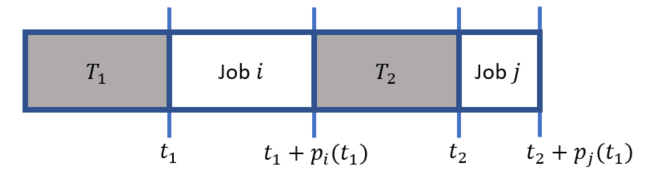
\includegraphics[width=\linewidth]{./assets/201802131917.PNG}
If we were to swap job $i$ and job $j$, we would get a new schedule, $S'$.\\
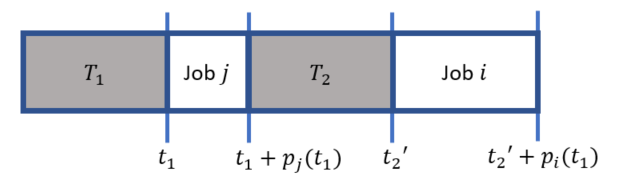
\includegraphics[width=\linewidth]{./assets/201802132355.PNG}
In this new schedule:
$$
\begin{aligned}
C_i&=t_1+p_i(t_1)\\
C_j&=t_2+p_j(t_1)\\
\vspace{1pt}\\
\sum_{k\in S} C_k&=\left(\sum_{k\in S/\{i,j\}}C_k\right)+C_i+C_j\\
&=(T_1+T_2)+(t_1+p_i(t_1))+(t_2+p_j(t_1))\\
\vspace{1pt}\\
\sum_{k\in S} C_k'&=\left(\sum_{k\in S/\{i,j\}}C_k'\right)+C_i'+C_j'\\
&=(T_1+T_2')+(t_2'+p_i(t_1))+(t_1+p_j(t_1))\\
\vspace{1pt}\\
\sum_{k\in S} C_k'-\sum_{k\in S} C_k&=T_2'-T_2+t_2'-t_2\\
\vspace{1pt}\\
T_2'&<T_2\\
t_2'&<t_2\\
\vspace{1pt}\\
\sum_{k\in S} C_k'-\sum_{k\in S} C_k &<0\\
\therefore \sum_{k\in S} C_k'&<\sum_{k\in S} C_k
\end{aligned}
$$
Therefore, schedule $S'$ is also optimal and also does not obey the SRFT rule.\\
\vspace{1pt}\\
As the new schedule does not follow the SRFT rule, there exists another pair of jobs $i$ and $j$ which the swap can be performed on.\\
This will result in an infinite set of schedules which are optimal.\\
\vspace{1pt}\\
As the set of optimal schedules is finite, the inverse statement must therefore be false, proving the original statement.
\pagebreak

\section{Question 3}
\textbf{Consider the problem $1|chains|\sum w_j(1-e^{-rC_j})$. Describe the algorithm that solves this problem and prove that it results in an optimal sequence.}
$$
\begin{aligned}
\textbf{Let  }\rho(1,\cdots,k)=\max_{l=1,\cdots,k}\frac{\sum_{j=1}^lw_j}{\sum_{j=1}^l(1-e^{-rC_j})}
\end{aligned}
$$
\begin{enumerate}[label=\textbf{Step \arabic{*}:}]
\item Evaluate $\rho(C_1,C_2,\cdots,C_n)$ where $\{C_1,C_2,\cdots,C_n\}$ is the set of all chains.
\item For the chain that corresponds to the $\rho$ value, examine the longest sub-chain that has the same $\rho$ value.
\item Append the sub-chain to the optimal sequence and return the remaining sub-chain to the set.
\item Repeat \textbf{Step 1-3} until no more chains remain.
\end{enumerate}
\pagebreak
\section{Question 4}
\textbf{Formulate the $1||\sum_jU_j$ scheduling problem where $U_j$ is equal to 1 if job $j$ is tardy. As an integer problem in the following three cases}
\begin{enumerate}[label=(\alph{*})]
\item \textbf{Completion time decision variables and disjunctive constraints}
$$
\begin{array}{crll}
\textbf{minimize}&\sum_{j=1}^nZ_j\\
\textbf{subject to}&C_j+p_k&\leq C_k+MX_{jk}&\forall j,k\\
&C_k+p_j&\leq C_j+M(1-X_{jk})&\forall j,k\\
&C_j-d_j&\leq MZ_j&\forall j\\
&C_j&\geq0&\forall j\\
&X_{jk}&\in\{0,1\}&\forall j,k\\
&Z_j&\in\{0,1\}&\forall j\\
\end{array}
$$
$$
\begin{array}{lrl}
\textbf{where}&X_{jk}=&\left\{\begin{array}{ll}1&\text{When }j\rightarrow k\\0&\text{Otherwise}\end{array}\right.\\
&Z_{j}=&\left\{\begin{array}{ll}1&\text{When job }j\text{ is tardy.}\\0&\text{Otherwise}
\end{array}\right.
\end{array}
$$
\item \textbf{Time-indexed decision variables}
$$
\begin{array}{crll}
\textbf{minimize}&\sum_{j=1}^{n}\sum_{t=1}^TZ_{jt}\\
\textbf{subject to}&\sum_{t=0}^TX_{jt}&=1&\forall j\\
&\sum_{j=1}^n\sum_{k=\max(0,t+1-p_j)}^tX_{jk}&\leq1&\forall j,t\\
&\sum_{t=0}^TX_{jt}(t-1+p_j-d_j)&\leq MZ_{jt}&\forall j,t\\
&X_{jt}&\in\{0,1\}&\forall j,t\\
&Z_{jt}&\in\{0,1\}&\forall j,t
\end{array}
$$
$$
\begin{array}{lrl}
\textbf{where}&X_{jt}=&\left\{\begin{array}{ll}1&\text{When job }j\text{ starts at time }t\\0&\text{Otherwise}\end{array}\right.\\
&Z_{j}=&\left\{\begin{array}{ll}1&\text{When job }j\text{ is tardy.}\\0&\text{Otherwise}
\end{array}\right.
\end{array}
$$
\item \textbf{Sequence-position decision variables}
$$
\begin{array}{crll}
\textbf{minimize}&\sum_{k=1}^nZ_k\\
\textbf{subject to}&\sum_{j=1}^nX_{jk}&=1&\forall k\\
&\sum_{k=1}^nX_{jk}&=1&\forall j\\
&C_{k-1}^*+\sum_{j=1}^np_jX_{jk}&\leq C_k^*&\forall k\\
&C_k^*-\sum_{j=1}^nd_jX_{jk}&\leq MZ_k&\forall k\\
&C_k^*&\geq0&\forall k\\
&X_{jk}&\in\{0,1\}&\forall j,k\\
&Z_k&\in\{0,1\}&\forall k
\end{array}
$$
$$
\begin{array}{lrl}
\textbf{where}&C_k^*:&\text{ Completion time of job at sequence position }k\\&X_{jk}=&\left\{\begin{array}{ll}1&\text{When job }j\text{ is assigned to position }k\\0&\text{Otherwise}\end{array}\right.\\
&Z_{j}=&\left\{\begin{array}{ll}1&\text{When job }j\text{ is tardy.}\\0&\text{Otherwise}
\end{array}\right.
\end{array}
$$
\end{enumerate}

\section{Question 5}
\textbf{Solve the $1|r_j|\sum_jw_jT_j$ scheduling problem with time-indexed variables in AMPL for the dataset provided.}
\begin{lstlisting}[language=AMPL]
CPLEX 12.8.0.0: optimal integer solution within mipgap or absmipgap; objective 139
4270685 MIP simplex iterations
1033392 branch-and-bound nodes
absmipgap = 0.000159996, relmipgap = 1.15105e-06
wT = 139 # Objective function value

C [*] := # Completion time values
 1   2
 2  18
 3   4
 4  19
 5  10
 6   9
 7   8
 8  15
 9  25
10  12
11  33
12  30
13  37
14  22
15   1
\end{lstlisting}
\pagebreak
\begin{appendix}
\section{Data file}
\lstinputlisting[language=AMPL]{./pset2.dat}
\section{Model file}
\lstinputlisting[language=AMPL]{./pset2.mod}
\section{Run file}
\lstinputlisting[language=AMPL]{./pset2.run}
\end{appendix}

\end{document}